\begin{figure}[ht]
    \centering
    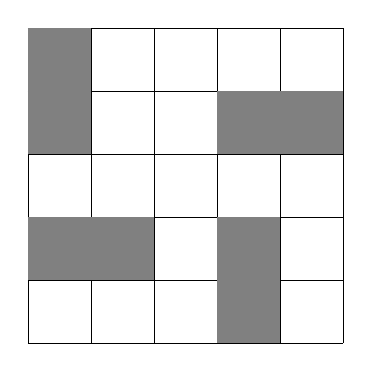
\begin{tikzpicture}[scale=0.8]
        \draw[step=1cm,ultra thin,black] (0,0) grid (5,5);

        \fill[gray] (1,1) rectangle ++(1,1);
        \fill[gray] (0,1) rectangle ++(1,1);
        \fill[gray] (3,3) rectangle ++(1,1);
        \fill[gray] (4,3) rectangle ++(1,1);
        \fill[gray] (0,3) rectangle ++(1,1);
        \fill[gray] (0,4) rectangle ++(1,1);
        \fill[gray] (0,4) rectangle ++(1,1);
        \fill[gray] (3,0) rectangle ++(1,1);
        \fill[gray] (3,1) rectangle ++(1,1);
    \end{tikzpicture}
    \caption{\centering Przykładowy wygląd końcowego, wygenerowanego labiryntu.}
    \label{fig:kruskal_example_maze}
\end{figure}